\chapter{実装}\label{chap:implementation_1}

本章ではその場に居合わせた人達の情報共有を可能にするサービス・アプリケーションの設計と実装および機能について述べる。

\newpage

\section{そこにいる名無しさんの実装}

ここでは、アプリケーションの詳細な実装および有する機能について述べる。

\subsection{概要}

その場に居合わせた人達が情報共有をするためのサービス・アプリケーションのプロトタイプとして"そこにいる名無しさん"を実装した。
本アプリケーションは、人々が普段持ち歩いている一般的なモバイルデバイスが持つBluetoothモジュールと連携することにより、
その場に居合わせた同じアプリケーションを持った人達との情報共有を可能にし、また後から見返すことができる。

Androidのスマートフォンデバイスと内蔵されたBluetoothモジュールを使用したアプリケーションを試作した。

本アプリケーションは、2012年のつながり展、SFC OpenResearchForum2012においてプロトタイプが展示され、
来場者からのフィードバックを得た後、2013年に改良を加えたものである。


\subsection{システム構成}

本アプリケーションは、大きくAndroid\cite{AndroidDevelopers}デバイス、APIサーバ、データベースの3つに分かれる。
クライアントはアプリケーションを起動することでアプリケーションはAndroidデバイスに常駐し、付近のBluetooth端末を検出する。
検出した場合、APIサーバにMACアドレスを自分のMACアドレスと共に送信する。
APIサーバは、データベースにそれぞれのMACアドレスの存在を確認するとともに、存在するMACアドレスに紐付けられたアクティビティをデータベースから取得する。
最後に、APIサーバはアクティビティインターフェイスのためにデータを加工した状態でクライアントにデータを返信する。
クライアントは、以上の処理が完了したのち、アクティビティを閲覧することが可能となる。
また、自身のアクティビティを更新するのはどの時点でも可能である。

APIサーバは著者の自宅にあるUbuntu12.04、機能はNode.js0.10で記述した。
データベースはMySQL5.5を使用している。

\begin{figure}[h]
    \begin{center}
        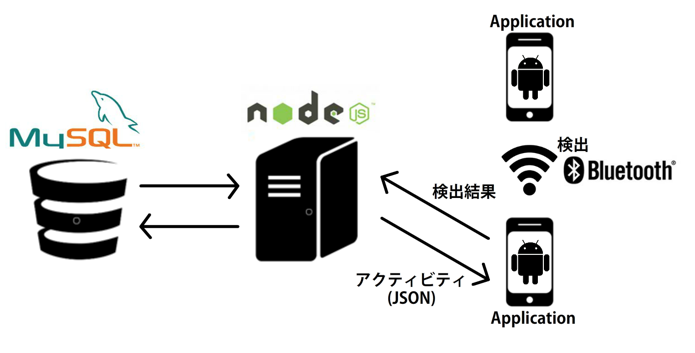
\includegraphics[width=1.0\linewidth]{img/servers.eps}
    \end{center}
    \caption{システム構成}
    \label{fig:servers}
\end{figure}

\newpage

\subsection{Androidアプリケーション}

プロトタイプを動作させる端末にはSamsung Galaxy NexusとASUS Nexus7 (2013)を使用した。
本アプリケーションで利用するBluetoothの機能は2.1のものであり、どちらとも機能要件を満たしている。
アプリケーションのソースコードはJavaで記述されている。

% 使用したデバイスに関するスペック表

\begin{table}[hb]
    \begin{center}
    \caption{Samsung Galaxy Nexus}

    \begin{tabular}{l|l}
        \hline
        OS & Android 4.0 \\
        画面サイズ & 4.7 インチ \\
        Bluetoothモジュール & Bluetooth 3.0 + EDR \\
        \hline
    \end{tabular}
    \end{center}
\end{table}

\begin{table}[hb]
    \begin{center}
        \caption{ASUS Nexus7 (2013)}

        \begin{tabular}{l|l}
            \hline
            OS & Android 4.3 \\
            画面サイズ & 7.02 インチ \\
            Bluetoothモジュール & Bluetooth 4.0 \\
            \hline
        \end{tabular}
    \end{center}
\end{table}

\newpage

\subsection{Bluetoothによるデバイス検出}

そこにいる名無しさんで実装に使用したAndroidデバイスでは、
周囲のBluetoothモジュールの検出にBluetooth2.1のプロトコルである検出機能を使用した。
検出を開始すると、およそ10秒間の間、周囲の検出可能なBluetoothモジュールを探索する。
検出可能なデバイスとは、あらかじめ自らを他のデバイスから検出可能な設定にしてあるBluetoothモジュールである。
Androidデバイスでは、デバイスのスキャンモードを検出可能(Discoverable)にすることで、行われる。

検出されたデバイスはBluetoothモジュールのMACアドレスが含まれるため、以降はこのMACアドレスをキーとしてデバイスを扱う。
これ以降に述べられる「MACアドレス」とは、全てBluetoothモジュールのMACアドレスのこととする。

一般的な携帯端末でのBluetooth検出効果範囲は10mである。検出の間、10m範囲内に検出可能なデバイスが含まれれば、検出結果に反映される。
10m以上に検出範囲を広げたい場合は、検出したデバイスが検出したデバイス、というようにデータを繋げていくことで実現可能となる。
これはホッピングと呼ばれ、Bluetooth MANETでは分散した機器が連携してデータをやりとりすることでホッピングを行うが、
本アプリケーションではBluetoothを近接デバイスの検出以上の機能は扱っていない。
ホッピングの機能は検出されたデバイスをサーバで管理することで、サーバ側での擬似的なホッピングを実装している。

検出可能なBluetoothモジュールは、探索の信号を受け取ると、レスポンスの信号を返すことにより、検出されることとなる。
また、Androidデバイスは、何も設定していない状態だと他のデバイスからの検出を無効にしている場合が多い。
今回使用した機種でもデフォルトでは無効の設定のため、アプリケーションはこの設定を監視し、常に有効にしている。


\subsection{サーバ・クライアントによる中央集権モデル}

Bluetoothを近接検出に利用した実装では、Bluetooth MANETを構築した分散モデルがある。
しかし、他のユーザーの投稿を扱う点で、それぞれのデバイスがデータを扱うのは、セキュリティ面で問題が残る。
本アプリケーションでは、後から投稿を閲覧する機能のために、サーバ・クライアントによる中央集権モデルを構築した。


\subsection{データベース・スキーマ}

データベースは、MySQLを使って実装されており、以下の3つのテーブルで構成される。

\begin{description}

\item{ユーザテーブル}

ユーザテーブルにはランダムに生成されたユニークなID情報をプライマリキーとして、
ユーザのBluetoothモジュールのMACアドレスが格納される。

\item{ユーザ検出テーブル}

ユーザ検出テーブルにはユーザが検出したMACアドレスのうち、
既にユーザテーブルに存在しているユーザ情報との結びつきが格納される。
格納される情報は、検出元のMACアドレス、検出されたMACアドレス、検出時間の3つである。

\item{ポストテーブル}

ポストテーブルには、ユーザが投稿したアクティビティが格納される。
格納される情報は投稿主であるユーザのMACアドレスと、
投稿の種類とその内容、投稿アクティビティのユニークIDである。
情報がメディアだった場合、blob形式で保存される。

\item{コメントテーブル}

コメントテーブルには、URL上から閲覧した人間がコメントを残した時にデータが格納される。
格納される情報は、コメント内容と、コメント先の投稿アクティビティが持つユニークなID、コメントが持つユニークなIDである。
コメントがメディアだった場合、blob形式で保存される。

\end{description}


\subsection{APIサーバ}

APIサーバは、クライアントからhttp通信で送られてきたデータを処理し、JSONフォーマットのデータ形式で返す役割を持っている。
APIサーバがインターフェイスとして持っているのは以下の3つである。

\begin{description}

\item{auth}

authは、クライアントがアプリケーション起動時にアクセスする場所で、ここではユーザの存在確認と認証を行う。
受け取ったユーザIDとMACアドレスをデータベースと照合し、ユーザの存在が確認できた場合はランダムな2つのユニーク色情報を生成して返す。
ここでMACアドレスのみを受け取った場合は、ランダムなユーザIDを生成後処理を行う。

\item{activity}

activityでは、ユーザIDと検出したMACアドレスの配列を受け取ってからMACアドレスがユーザテーブルに存在するか確認をとる。
存在していた場合はユーザ検出テーブルに検出元と検出されたユーザIDが現在時刻とともに挿入される。
検出されたユーザIDはユーザ検出テーブルから更に、検出されたユーザが10分以内に検出したユーザIDを取得する。
アプリケーションではこの操作をサーバ内での擬似的なホッピングと呼んでいる。
擬似ホッピングを3回行った後、一覧を重複のないユニークな一覧に整列した後、ポストテーブルから過去のアクティビティを取得する。
アクティビティは擬似ホッピングの際に計算された重複度の高い順に整列され、
ユーザの色ID情報を付加した後、JSONデータ形式でクライアントに返される。

\item{post}

postは、クライアントからユーザIDと投稿されたアクティビティを受け取る場所である。
受け取った情報は現在時刻と投稿固有のランダムなIDを付加された後、ポストテーブルに挿入される。

\item{get}

getでは、ユーザが投稿したアクティビティデータを扱う。
この場所だけは、JSONではなくHTMLデータを表示するビューが存在する。
get/[post ID]のようなURLでアクセスした時に、投稿されたアクティビティが単独で表示されるようになっている。
URLはアクティビティが投稿された際に生成される。
このURLは永続的なもので、URLを知っている人間はWebブラウザ上からアクティビティを閲覧することが可能である。
また、このページからはアクティビティへのコメント付加も可能である。

\item{comment}

commentでは、getの画面でPOSTメソッドによりコメントされたデータを扱う。
データはコメントテーブルに格納され、以降コメント対象となったアクティビティのページでコメントが閲覧できる。

\end{description}


\subsection{インターフェイス}

アプリケーションの初期画面インターフェイスは、チャットアプリケーションのタイムライン画面に似たデザインをしている。
アクティビティ画面、アクティビティの投稿画面はWebviewコンポーネントで表示しており、
インターフェイスに関わるソースコードはHTML, CSS, Javascriptによって記述されている。
サーバから受け取ったJSONデータはWebviewコンポーネントに受け渡され、Javascriptがデータを整形して表示する。

\subsection{アクティビティの投稿}

ユーザはアプリケーションの右上のボタンから、
自分のアクティビティを投稿することができる。
投稿されたアクティビティは、自分のデバイスを検出したユーザのアクティビティ画面と、
自分自身のアクティビティ画面に反映される。

またユーザはクライアントのアクティビティ投稿画面から、
文字だけでなくメディアファイルを共有することが可能である。

共有するメディアはアプリケーションサーバにアップロードされ、
アクティビティ画面にはメディアファイルへのリンクとして表示される。

\subsection{ブラウザからの投稿されたアクティビティの閲覧}

クライアントのアクティビティ画面から個別の投稿をタッチすると、ブラウザへのインテントが発生する。
インテントは、文字列の情報を指定したアプリケーションへ送信するAndroidの仕組みである。
ここでは、ブラウザに投稿されたアクティビティへのURLが受け渡され、
ユーザはブラウザから個別に投稿を閲覧することが可能となる。

\begin{figure}[hp]
  \begin{center}
    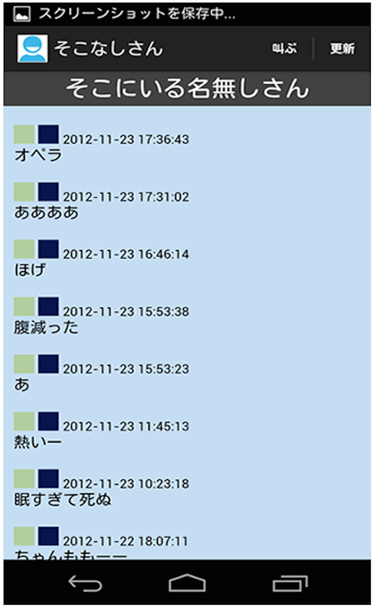
\includegraphics[width=0.5\linewidth]{img/v1_visual.eps}
  \end{center}
  \caption{インターフェイス}
  \label{fig:interface}
\end{figure}

\begin{figure}[t]
  \begin{center}
    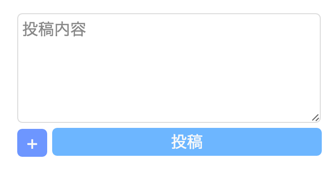
\includegraphics[width=0.5\linewidth]{img/post.eps}
  \end{center}
  \caption{投稿フォーム}
  \label{fig:post}
\end{figure}

\begin{figure}[t]
  \begin{center}
    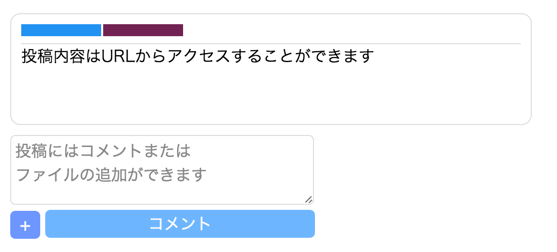
\includegraphics[width=0.8\linewidth]{img/get.eps}
  \end{center}
  \caption{ブラウザから見た投稿}
  \label{fig:get}
\end{figure}
